\documentclass[12pt]{article}
\usepackage[english]{babel}
\usepackage[utf8x]{inputenc}
\usepackage{amsmath}
\usepackage{tikz}
\usetikzlibrary{arrows,automata}
\begin{document}
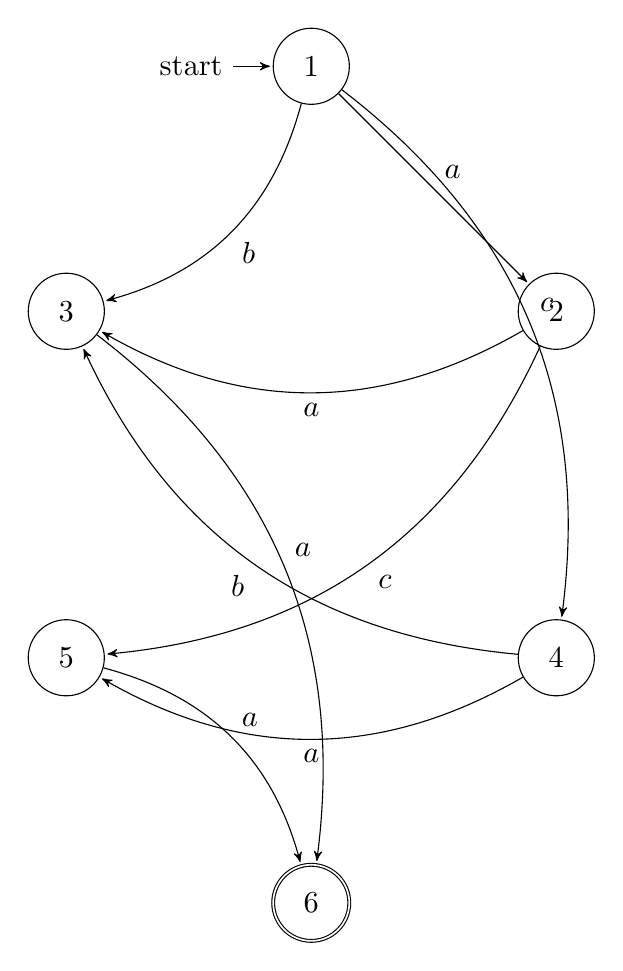
\begin{tikzpicture}[->,>=stealth',shorten >=1pt,auto,node distance=4cm, scale = 1.1,transform shape]
\node[state,initial] (0)   {$1$};
\node[state]  (1) [below right of = 0] {$2$};
\node[state]  (2) [below left of = 0] {$3$};
\node[state]  (3) [below of = 1] {$4$};
\node[state]  (4) [below of = 2] {$5$};
\node[state,accepting] (5) [below right of = 4] {$6$};
\path (0) edge node {$a$}(1)
   (0) edge [bend left] node {$b$}(2)
   (0) edge [bend left] node {$c$}(3)
   (1) edge [bend left] node {$a$}(2)
   (1) edge [bend left] node {$c$}(4)
   (2) edge [bend left] node {$a$}(5)
   (3) edge [bend left] node {$a$}(4)
   (3) edge [bend left] node {$b$}(2)
   (4) edge [bend left] node {$a$}(5)
;
\end{tikzpicture}
\end{document}
